\chapter{Introduction}
\label{ch:introduction}

\dictum[Dante Alighieri]{%
  Abandon all hope, ye who enter here. }%
\vskip 1em

\readit{2}

% \worktodo{
%    * we focus on these publications (MG LMA, GPU stuff, not cstar HVP stuff)
%    * motivation (1-2 pages)
%    * intro in lattice field theory (fundamentals)
%    * action, O(a) improvement
%    * Cstar, QCD+QED
%    * Dirac operator; already done in p2 intro
%    * fix the physical point
%    * fix the scale, 
%    * recover the continuum limit
% * GPUs
% * noise reduction methods
%    * scope of this work
%    * Structure of the thesis: Part 1 deal with the GPU stuff, part2 the algorithmic improvement noise reduction and stuff
%    * overall 5-10 pages
%    * topics: lattice field theory intro, dirac op, QCD+QED, C*, (first 2 pages of GPU-intro), (first page g-2 intro), Research problem and objectives, Summary of Contributions, non-perturbative treatment necessary, only ab initio method for non-perturbative access to QCD, Structure of the thesis
% }

The standard model of particle physics is one of the most successful frameworks for theoretical predictions of physical quantities.
Its agreement with experimental data is unprecedented.
%Lattice field theory (LFT) is still the only regularization of quantum field theory (QFT) and by this the only ab initio method that allows non-perturbative access to observables.
Lattice field theory is currently the only non-perturbative regularization of quantum field theory that allows for the numerical computation of non-perturbative observables from first principles.
%Due to its statistical nature, determinations from lattice field theory can be systematically improved.
Moreover, determinations from lattice field theory can be systematically improved.
Gold-plated observables like the anomalous magnetic momentum of the muon $g-2$, where low energy behavior of QCD plays an important role are accessible from basic principles only non-perturbatively with the application of lattice QCD and QED.
When adopting lattice regularization, the fields of the continuum theory are discretized in spacetime and represented as degrees of freedom associated to sites and links in a four dimensional spacetime hypercube.
The discretization of the theory naturally regularizes ultraviolet and infrared divergences occurring in the continuum theory, due to its finite resolution and volume description.
Feynman's path integral description of QFT is used as a representation, where the functional integral over field degrees of freedom turns into a high-dimensional regular integral.
%Dimensionality may go up to $10^{8}$, which introduces the need of modern high-performance computing (HPC) infrastructure for their evaluation.
A typical lattice QCD ensemble, with a volume on the order of a few fermi and lattice spacings well below \num{1} fermi\footnote{To simulate nucleons for instance, one requires lattice extents of a few fermi because the nucleon radius is about \num{1} fm, whereas the lattice spacing must be significantly smaller than that to give a proper resolution.}, contains at least $\bigO(10^8)$ degrees of freedom, including flavors, colors, and space-time indices.
This introduces the need of modern high-performance computing (HPC) infrastructure for their evaluation.
Careful understanding of systematic and statistical errors allows studying physical quantities of interest and thorough comparison to experiment.
\worktodo{Tim: Maybe you go into this later, but it would be nice to go into a bit more depth here.}
Discretizing a theory comes with many decisions and choices; each with its advantages and disadvantages.
Independent research groups in the field, working with different discretizations, regularly compare their results and discuss systematics.
Once extrapolated to the continuum, lattice results should show independence of these choices and agree within their error estimates -- this is often called universality.

\section{Fundamentals of lattice field theory}

As already touched upon, lattice field theory is a discretized version of continuum quantum field theory.
%As introduced by Feynman in 1948~\cite{Feynman1948}, expectation values of observables in context of continuum quantum field theory can be mathematically represented as functional integrals over the involved fundamental fields
Expectation values of observables in the context of continuum quantum field theory can be mathematically represented as functional integrals over the involved fundamental fields~\cite{Feynman1948}
\begin{equation} \label{eq:path:integral:expectation:value}
\langle \observable{O}[\psi, \bar{\psi}, A] \rangle =
\frac{1}{Z} \int
\DD \psi
\DD \bar{\psi}
\DD A \;
\observable{O}[\psi, \bar{\psi}, A]
e^{i S[\psi, \bar{\psi}, A]} \;.
\end{equation}
In this equation, the fundamental degrees of freedom are the fields $\psi$, $\bar{\psi}$ and $A$.
$S$ denotes the action of the theory and $Z = \int \DD \psi \DD \bar{\psi} \DD A e^{i S[\psi, \bar{\psi}, A]}$ the partition function.
The observable $\observable{O}$ is a functional of the fields and can be any time-ordered correlation function.
Here, $\psi$ and $\bar{\psi}$ may represent fermionic particles and $A$ a gauge boson.
The bosonic field is vectorial and the fermionic one spinorial and Grassmann-valued.
It is a standard result in fermionic QFT that the fermion degrees of freedom in the partition function $Z$ can be integrated out, such that
\begin{equation}
Z = \int \DD A \det(D) e^{i S[A]} \;.
\end{equation}
The non-locality of the determinant encodes all possible paths of the fermion represented by $\psi$.
For the first time, we encounter the operator that has a central role in this document; the Dirac operator $D$, here in its continuum form $D = i \gamma^{\mu} D_{\mu} - m$ with the Dirac matrices obeying the Clifford algebra $\{\gamma^{\mu}, \gamma^{\nu}\} = 2 \eta^{\mu \nu}$, where $\eta$ is the Minkowski spacetime metric\footnote{In particle physics notation usually of signature $(+---)$.}, $m$ is the fermion mass and $D_{\mu}$ are covariant derivatives
\begin{equation}
D_{\mu} = \partial_{\mu} + ig A_{\mu}^{a} T^{a} \;,
\end{equation}
where the $T^{a}$ are the generators of the gauge group's Lie-algebra and $g$ the coupling.
These derivatives were introduced to retain Lorentz-invariance of the kinetic fermion part of the action $S$.
Inevitably, this introduced another field $A$ which is vector-valued, massless and mediates the interaction among fermions.
In the context of QED with gauge group $\ggrp{U}{1}$, this results in the photon mediating the electromagnetic interaction, whereas for an $\ggrp{SU}{3}$ gauge group this results in the \num{8} gluons mediating the strong interaction of quantum chromodynamics (QCD).

The fermionic quark fields belong to the $N_c$-dimensional fundamental representation of the color gauge group $\ggrp{SU}{N_c}$, antiquark fields to the complex conjugate representation of $\ggrp{SU}{N_c}$ which is $N_c$-dimensional too, and gluon fields to the adjoin representation which is $N_c^{2}-1$ dimensional.

In order to identify \cref{eq:path:integral:expectation:value} with a classical statistical model, we have to perform a Wick-rotation translating Minkowski into Euclidean spacetime, $t_m \to -i t_e$, where $t_m$ is the \emph{real} Minkowski time and $t_e$ is the (real valued) Euclidean time.
The effect of this on the action is that $e^{i S_m}$ turns into $e^{- S_e}$ allowing the interpretation of the Euclidean action $S_e$ which is real (for zero chemical potential) as a Boltzmann weight in a statistical sense as opposed to the oscillatory behavior of the Minkowski action exponential $e^{i S_m}$.
This poses no problem, since Euclidean correlation functions can be analytically continued to Minkowski space preserving physical contents of the theory~\cite{Osterwalder:1974tc} and vice versa.
Due to this rotation, correlation functions on the lattice $C(t_e)$, have to be interpreted with Euclidean time.
\worktodo{Tims comment}
Euclidean time evolution is thus exponentially decaying as opposed to oscillatory in Minkowski space,
\begin{align}
C(t_e) &= \sum_n A_n e^{ - E_n t_e} \;, &\makebox[\widthof{\text{(Minkowski)}}][l]{\text{(Euclidean)}} \\
C(t_m) &= \sum_n A_n e^{-i E_n t_m} \;. &\text{(Minkowski)}
\end{align}

The Euclidean theory can be discretized by introducing a finite four dimensional spacetime lattice $\Lambda$ of Cartesian coordinates.
Lattice sites are evenly spaced by the dimensionful lattice spacing $a$ such that the coordinates are dimensionless.
We write fields defined on the lattice in resemblance of their continuum analogues as $\psi(x)$ with $x=an$, $n \in \Lambda$ a dimensionless, non-negative integer, subject to boundary conditions.
The lattice spacing $a$ provides the finite resolution of the discretization curing UV divergences with a momentum cutoff proportional to $1/a$ and the finite lattice volume $V = \lvert \Lambda \rvert$ cures IR divergences with a cutoff proportional to $a$.
This provides a natural regularization of continuum theory.

Fermion fields are defined on the lattice sites with possible further \emph{internal} degrees of freedom for spin and color, whereas gauge fields acting as parallel transports linking neighboring lattice sites, are imagined to live in between sites.
Depending on the gauge group, gauge links possess further internal degrees of freedom with values drawn from the gauge group.

The dynamics of the theory are governed by the continuum QCD action~\cite{yangmills1954}
\begin{equation} \label{eq:continuum:YM:action}
S = \int \dd x \; \mathcal{L}(x) \;,
\quad
\mathcal{L}(x) = - \frac{1}{4} F^{a}_{\mu \nu}(x) F_{a}^{\mu \nu}(x) + \bar{\psi}(x) (D \psi)(x) \;,
\end{equation}
with the continuum Dirac operator $D$ and the Yang-Mills field strength tensor
\begin{equation}
F_{\mu \nu}^{a}(x) = \partial_{\mu} A_{\nu}^{a}(x) -\partial_{\nu} A_{\mu}^{a}(x) + g f^{abc} A_{\mu}^{b}(x) A_{\nu}^{c}(x) \;.
\end{equation}
The coupling constant $g$ is a free parameter of the theory and the structure constants $f^{abc}$ parametrize the Lie-algebra of the gauge group.

\subsection{Dirac operator}

Discretizing the QCD action \cref{eq:continuum:YM:action} and replacing derivatives with symmetric differences results in the Wilson action~\cite{Gattringer:2010zz}
\begin{align}
S &= S_G + S_F \;, \\
S_G &= \frac{1}{g^2} \sum_{x \in a \Lambda} \sum_{\mu, \nu} \Re \tr \left[ \delta_{\mu \nu} \id - U_{\mu \nu}(x) \right] \;, \label{eq:wilson:action:gauge} \\
S_F &= a^4 \sum_{x \in a \Lambda} \bar{\psi}(x) (D_{\text{naive}}[U] \psi)(x) \;.
\end{align}
The gauge part of the action $S_G$ turns into a sum over plaquettes (see \cref{fig:plaquette} for an illustration)
\begin{equation} \label{eq:plaquette}
U_{\mu \nu}(x)
= U_{\mu}(x) U_{\nu}(x + \hat{\mu}) U_{\mu}(x + \hat{\nu})^{\dagger} U_{\nu}(x)^{\dagger} \;,
\end{equation}
where $U_{\mu}$ is the Lie-group-valued gauge field
\begin{equation} \label{eq:gauge:field}
U_{\mu}(x)
= P \exp(i g \int_x^{x + a \hat{\mu}} \dd z_{\mu} A_{\mu}(z) )
\approx e^{i g a A_{\mu}(x + \frac{a}{2} \hat{\mu})} \;,
\end{equation}
as exponential of the Lie-algebra-valued field $A$ and $\hat{\mu}$ is the unit 4-vector in direction $\mu$.
As constructed in \cref{eq:gauge:field}, gauge links are explicitly defined in between lattice sites.
The fermion part $S_F$ introduces the discretized Dirac operator -- the naive lattice Dirac operator
\begin{equation}
% (D \psi)(x) = (4+m)\psi(x) \\
% + \frac{1}{2} \sum_{\mu} \left\{
%   (1 - \gamma_{\mu}) U_{\mu}(x) \psi(x + \hat{\mu}) + (1 + \gamma_{\mu}) U_{\mu}(x - \hat{\mu})^{-1} \psi(x - \hat{\mu})
% \right\} \;.
D_{\text{naive}}[U] = m + \frac{1}{2} \sum_{\mu} \gamma_{\mu} \left( D_{+\mu} + D_{- \mu} \right) \;,
\end{equation}
with the discretized covariant forward and backward derivatives
\begin{align}
%D_{+ \mu}(x,y) &= \frac{1}{a} \left[ U_{\mu}(x) \delta_{x+\hat{\mu},y} - \delta_{x,y} \right] \;, \\
%D_{- \mu}(x,y) &= \frac{1}{a} \left[ \delta_{x,y} - U_{\mu}(x - \hat{\mu})^{\dagger} \delta_{x - \hat{\mu}, y} \right] \;, \\
%D_{+ \mu} &= \frac{1}{a} \left[ U_{\mu} T_{\mu} - \id \right] \;, \\
%D_{- \mu} &= \frac{1}{a} \left[ \id - U_{-\mu} T_{-\mu} \right] \;, \\
%D_{\pm \mu} &= \pm \frac{1}{a} \left[ U_{\pm \mu} T_{\pm \mu} - \id \right] \;, \\
D_{\pm \mu}(x,y) &= \pm \frac{1}{a} \left[ U_{\pm \mu}(x) \delta_{x \pm \hat{\mu}, y} - \delta_{x,y} \right] \;,
%D_{+ \mu} f(x) &= \frac{1}{a} \left[ U_{\mu}(x) f(x + \hat{\mu}) - f(x) \right] \;, \\
%D_{- \mu} f(x) &= \frac{1}{a} \left[ f(x) - U_{\mu}(x - \hat{\mu})^{\dagger} f(x - \hat{\mu}) \right] \;,
\end{align}
and the $\gamma_{\mu}$ are the Dirac matrices obeying the Euclidean Clifford algebra $\{\gamma_{\mu}, \gamma_{\nu}\} = 2 \delta_{\mu \nu}$.

Since the gauge field lives on the links between lattice points, the parallel transporter in positive direction $\mu$, linking point $x$ with its neighbor $x + \hat{\mu}$, is related to the link in negative $\mu$ direction linking point $x + \hat{\mu}$ and $x$ by Hermitian transpose.
For $\mu=1,2,3,4$ a direction, this results in
\begin{equation}
U_{\pm \mu}(x) = U_{\mp \mu}(x \pm \hat{\mu})^{\dagger} \;,
\end{equation}
where $\pm$ denotes the link in positive or negative $\mu$-direction, respectively.

When expanding in $a$, we find that the naive gauge action \cref{eq:wilson:action:gauge} has $\bigO(a^{2})$ discretization effects
\begin{equation}
\frac{1}{g^2} \Re \tr \left[ \delta_{\mu \nu} \id - U_{\mu \nu}(x) \right] = \frac{1}{2} \tr\left[ F_{\mu \nu}^{a}(x) F_{\mu \nu}^{b}(x) T^{a} T^{b} \right] + \delta_{\mu \nu} \bigO(a^{2}) \;.
\end{equation}
The naive Dirac operator introduces fermion doublers; unphysical poles in the fermion propagator $(D_{\text{naive}})^{-1}$.
These correspond to particles that do not exist in continuum theory.
%and the doublers make the operator ill-conditioned in general \worktodo{ref}, unsuitable for numerical studies.
The Dirac operator can be extended by any term proportional to the lattice spacing $a$ or positive powers thereof; such a term will vanish when taking the continuum limit $a \to 0$.
Wilson himself proposed a solution to the fermion doubling problem~\cite{PhysRevD.25.2649} resulting in the Wilson-Dirac operator
\begin{equation} \label{eq:dirac:wilson}
D_W[U] = D_{\text{naive}}[U] - \frac{a}{2} \sum_{\mu} D_{-\mu} D_{+\mu} \;.
\end{equation}
The additional Wilson-term proportional to $a$ removes the fermion doubler states by adding a term proportional to $1/a$ to their masses.
Such states decouple in the continuum limit, but the term above breaks chiral symmetry and introduces $\bigO(a)$ discretization errors.
Even more troubling, every discretization with the correct continuum limit and respecting locality, either comes with fermion doublers or breaks chiral symmetry.
This is the famous Nielsen-Ninomiya no-go theorem~\cite{Nielsen:1980rz,Nielsen:1981xu}.

An additional term proportional to $a$ was introduced later to cancel the $\bigO(a)$ discretization effects introduced by the Wilson-term systematically, while still eliminating the doublers,
\begin{equation} \label{eq:dirac:wilson:clover}
D_{WC}[U] = D_W[U] + c_\mathrm{sw}^{SU(3)} a \frac{i}{4} \sum_{\mu, \nu} \sigma_{\mu \nu} \hat{F}_{\mu \nu} \;.
\end{equation}
This is called the Wilson-Clover Dirac operator.
Here, $\sigma_{\mu \nu} = \frac{i}{2} \left[\gamma_{\mu}, \gamma_{\nu}\right]$ and the discretized $SU(3)$ field strength tensor $\hat{F}_{\mu \nu}$ is defined as
\begin{align}
\hat{F}_{\mu \nu}(x) &= \frac{1}{8} \left\{
    Q_{\mu \nu}(x) - Q_{\nu \mu}(x)
\right\} \;, \label{eq:intro:clover} \\
Q_{\mu \nu}(x)
&= U_{\mu}(x)
   U_{\nu}(x+\hat{\mu})
   U_{\mu}(x+\hat{\nu})^{-1}
   U_{\nu}(x)^{-1} \label{eq:intro:clover:p1} \\
&+ U_{\nu}(x)
   U_{\mu}(x-\hat{\mu}+\hat{\nu})^{-1}
   U_{\nu}(x-\hat{\mu})^{-1}
   U_{\mu}(x-\hat{\mu}) \label{eq:intro:clover:p2} \\
&+ U_{\mu}(x-\hat{\mu})^{-1}
   U_{\nu}(x-\hat{\mu}-\hat{\nu})^{-1}
   U_{\mu}(x-\hat{\mu}-\hat{\nu})
   U_{\nu}(x-\hat{\nu}) \label{eq:intro:clover:p3} \\
&+ U_{\nu}(x-\hat{\nu})^{-1}
   U_{\mu}(x-\hat{\nu})
   U_{\nu}(x+\hat{\mu}-\hat{\nu})
   U_{\mu}(x)^{-1} \;. \label{eq:intro:clover:p4}
\end{align}
The term proportional to $c_\mathrm{sw}^{SU(3)}$ is called the clover- or SW-term and was proposed by Sheikholeslami and Wohlert~\cite{sw1985} as addition to the action, see \cref{fig:clover} for an illustration.
It is block-diagonal.
Following an effective field theory analysis it gives $\bigO(a)$ improvement à la Symanzik~\cite{symanzik1982,SYMANZIK1983} by tuning the algorithmic parameter non-perturbatively $c_\mathrm{sw}^{SU(3)}$ such that $\bigO(a)$ discretization effects vanish~\cite{LUSCHER1996365}.
%Furthermore, the clover-term has a positive impact on the numerical condition.
%\worktodo{check last sentence in chirality chapter}

\begin{figure}
\centering
\subfloat[The plaquette]{%
  \includestandalone[width=0.5\textwidth]{\dir/img/plaquette}
  \label{fig:plaquette}
}
\hfill
\subfloat[The clover term]{%
  %\includestandalone[width=0.45\textwidth]{\dir/img/clover}
\resizebox{0.3\textwidth}{!}{%
\begin{tikzpicture}

\tikzset{
  gauge/.style = {
    shorten <=9pt,
    shorten >=9pt,
    color=black,
    postaction={
      decorate,
      decoration={
        markings,
        mark=at position 0.5 with {\arrow{Stealth}}
      }
    }
  },
  point/.style = {
    color=black
  }
}

\fill[point] (0,0)   circle (0.05);
\fill[point] (3,0)   circle (0.05);
\fill[point] (6,0)  circle (0.05);

\fill[point] (0,3)   circle (0.05);
\fill[point] (3,3)   circle (0.05) node[below]  {$x$};
\fill[point] (6,3)  circle (0.05);

\fill[point] (0,6)  circle (0.05);
\fill[point] (3,6)  circle (0.05);
\fill[point] (6,6) circle (0.05);

\draw[gauge] (0,0.15) -- (3,0.15);
\draw[gauge] (2.85,0) -- (2.85,3);
\draw[gauge] (3,2.85) -- (0,2.85);
\draw[gauge] (0.15,3) -- (0.15,0);

\draw[gauge] (3,0.15) -- (6,0.15);
\draw[gauge] (5.85,0) -- (5.85,3);
\draw[gauge] (6,2.85) -- (3,2.85);
\draw[gauge] (3.15,3) -- (3.15,0);

\draw[gauge] (0,3.15) -- (3,3.15);
\draw[gauge] (2.85,3) -- (2.85,6);
\draw[gauge] (3,5.85) -- (0,5.85);
\draw[gauge] (0.15,6) -- (0.15,3);

\draw[gauge] (3,3.15) -- (6,3.15);
\draw[gauge] (5.85,3) -- (5.85,6);
\draw[gauge] (6,5.85) -- (3,5.85);
\draw[gauge] (3.15,6) -- (3.15,3);

%\draw[->] (-3,0) -- (-2,0) node[midway, below] {$\mu$};
%\draw[->] (-3,0) -- (-3,1) node[midway, left]  {$\nu$};

\node[anchor=center] at (4.5,4.5) {\cref{eq:intro:clover:p1}};
\node[anchor=center] at (1.5,4.5) {\cref{eq:intro:clover:p2}};
\node[anchor=center] at (4.5,1.5) {\cref{eq:intro:clover:p4}};
\node[anchor=center] at (1.5,1.5) {\cref{eq:intro:clover:p3}};

\end{tikzpicture}%
}
\label{fig:clover}
}
\caption{
Illustration of the plaquette term (left) which is a matrix-matrix product of gauge links along the lines as in \cref{eq:plaquette} and the clover term (right) which is a sum of rotated plaquettes that resemble the form of a clover leaf. The individual plaquettes correspond to the summands in \cref{eq:intro:clover:p1,eq:intro:clover:p2,eq:intro:clover:p3,eq:intro:clover:p4}.
}
\label{fig:plaquette:clover}
\end{figure}

There are many alternative discretizations to the above.
All deal differently with chiral symmetry on the lattice and the doubling problem.
Staggered fermions~\cite{PhysRevD.11.395} reduce the \num{16} doublers to \num{4} \emph{tastes} and retain a remnant \ggrp{U}{1} chiral symmetry.
Domain-wall fermions~\cite{Kaplan:1992bt,Shamir:1993zy} suppress doublers through the introduced fifth dimension of extent $L_s$ and exact chiral symmetry is obtained in the limit\footnote{Typically $L_s$ is chosen to be around \numrange{12}{48}.} $L_s \to \infty$.
Twisted-mass fermions~\cite{Frezzotti:2000nk} remove doublers with the Wilson term and chiral symmetry breaking effects are improved by the mass twisting.
Overlap fermions~\cite{Neuberger:1997fp,Neuberger:1998wv} entirely remove doublers and retain exact chiral symmetry.
This is in agreement with Nielsen-Ninomiya~\cite{Nielsen:1980rz,Nielsen:1981xu}, because their Dirac operator is non-local (but exponentially local~\cite{Hernandez:1998et,Boyle:2016imm}) making it computationally very expensive.

Summarizing, the QCD Wilson-Clover Dirac operator -- which for simplicity we will call $D$ in the remainder of this document -- is a nearest-neighbor stencil operator acting on a linear space of quark (or spinor) fields defined on a regular 4D cubic lattice of $V$ sites, typically in the range $10^6-10^8$.
Applied to a spinor field $\psi(x)$ the Dirac operator can then be written as a stencil (the lattice spacing is set to $a = 1$)
\begin{equation}
\begin{aligned} \label{eq:Dw}
(D &\psi)(x) = (4 + m) \psi(x) \\
-&\frac{1}{2} \sum_{\mu=0}^3 \Big\{
  U_{\mu}(x) (1-\gamma_{\mu}) \psi(x + \hat{\mu})
+ U_{\mu}(x-\hat{\mu})^{-1} (1+\gamma_{\mu}) \psi(x-\hat{\mu})
\Big\} \\
+&c_\mathrm{sw}^{SU(3)} \frac{i}{4} \sum_{\mu,\nu=0}^3 \sigma_{\mu \nu} F_{\mu \nu}(x) \psi(x),
\end{aligned}
\end{equation}
where the gauge field $U_{\mu}(x)$ is the $SU(3)$-valued link between lattice points $x$ and $x + \hat{\mu}$.
The term $4+m = \frac{1}{2 \kappa}$ where $\kappa$ is the inverse mass.

Notable about this choice of discretization are some properties which we briefly review here, because they will become important later.
The operator has the property of pseudo-Hermiticity with respect to $\gamma^5 = \gamma_0 \gamma_1 \gamma_2 \gamma_3$, $D^{\dagger} = \gamma^{5} D \gamma^{5}$.
Among many implications (as discussed later), its eigenvalues are either real or come in complex conjugate pairs and its determinant is real.

\subsection{Dirac equation}

Due to the nearest-neighbor coupling, a good parallelization scheme is achieved by domain decomposition, where a contiguous local volume of size $V_\mathrm{L}=L_0 L_1 L_2 L_3$, which divides the global problem size, is associated with a single compute unit.
With increasing problem sizes, the Dirac operator is poorly conditioned and sophisticated preconditioning algorithms are required to obtain acceptable convergence rates of iterative solvers.

\tldr{Definition of Dirac eq on lattice}
The system of linear equations of interest is the Dirac equation
\begin{equation} \label{eq:dirac:equation}
  D \psi = \eta \;,
\end{equation}
where different choices for the right-hand side $\eta$ result in different propagator expressions.
Solves of this equation appear repeatedly throughout the field and will be a central computational, algorithmic and theoretical motive throughout this thesis.

\subsection{Lattice expectation values}

Taking our previous considerations into account, we find for Euclidean expectation values
\begin{equation} \label{eq:eclidean:exp:value}
\langle \observable{O}[\psi, \bar{\psi}, U] \rangle =
\frac{1}{Z}
\int \DD U
\det(D) e^{- S_G[U]}
\observable{O}[U] \;.
\end{equation}
The integral measure $\DD U$ is the Haar measure~\cite{haar1933} of the group manifold.
Fermion field dependencies of the observable in the integrand $\observable{O}[U]$ are Wick-contracted and replaced by traces over fermion propagators $D^{-1}$ from lattice points $x$ to $y$.
The observable now depends on solutions to the Dirac equation $D[U] \phi = \eta$, rather than the numerically inaccessible Grassmann-valued fermion fields $\psi(x)$ and $\bar{\psi}(x)$\footnote{This is a pattern occurring repeatedly in the field. As soon as fermions are introduced, expressions become non-local, like the determinant when integrating out the fermion fields or the appearance of $D^{-1}$ when Wick-contracting. This is the price to pay for a proper numerical treatment of Pauli's exclusion principle in Lagrangian field theory dynamics. A similar process happens in Hamiltonian dynamics where the boomerang might hit even harder since the Jordan-Wigner transformation is non-local.}.

The expectation value in its Euclidean form \cref{eq:eclidean:exp:value} is now amenable for numerical evaluation using Monte Carlo simulations.
We can define a probability density function for the gauge fields as
\begin{equation} \label{eq:prob:density}
P(U) = \frac{1}{Z} \det(D) e^{- S_G[U]} \;,
\end{equation}
importance sample a set of $\Nconf$ gauge fields according to it $\{U_i\}_{i=1}^{\Nconf}$ and estimate the expectation value of the observable as a mean over the samples
\begin{equation}
\langle \observable{O}[\psi, \bar{\psi}, U] \rangle \approx \frac{1}{\Nconf} \sum_{i=1}^{\Nconf} \observable{O}[U_i]
\end{equation}
with variance $\observable{O}^{2} / N$.


\subsection{Monte Carlo sampling}

% \worktodo{
%    * Hybrid Monte Carlo (HMC)
%    * Markov chain
%    * ergodicity
%    * accept-reject
%    * Metropolis
% }

For the remaining integral over the gauge field in \cref{eq:eclidean:exp:value} Markov Chain Monte Carlo methods are usually to sample the integral\footnote{The field is very active in finding cheaper alternative solutions to this. Machine learning and AI are promising candidates.}.
According to the probability density \cref{eq:prob:density}, sampling algorithms generate a Markov chain of so called \df{gauge field configurations}.
It is challenging for the Markov process to satisfy ergodicity~\cite{10.1063/5.0004106,PhysRevLett.60.1243} (all configurations can be reached) and detailed balance (probability flow into a configuration equals the flow out).

With dynamical fermions in lattice field theory, most common is the Hybrid Monte Carlo algorithm~\cite{DUANE1987216} (HMC).
It introduces conjugate momentum variables $\pi$ and defines a fictitious Hamiltonian that depends on the gauge field and its conjugate variable
\begin{equation}
\mathcal{H}[U, \pi] = \frac{1}{2} \pi^{2} + S_{G}[U] + \phi^{\dagger} (D^{\dagger} D)^{-1} \phi \;.
\end{equation}
The pseudofermion field $\phi$ was introduced to stochastically represent the determinant $\det(D^{\dagger} D)$.
In this case we simulate two degenerate quark flavors\footnote{For a single flavor usually Rational HMC (RHMC) is used, where $\det(D) \sim \int \DD \phi^{\dagger} \DD \phi e^{-\phi^{\dagger} R(D) \phi}$ with $R(D) \approx D^{-1}$ a rational function approximation to $D^{-1}$.}.
This comes from the standard Gaussian integral formula
\begin{equation}
\det(D^{\dagger} D) \sim \int \DD \phi^{\dagger} \DD \phi e^{- \phi^{\dagger} ( D^{\dagger} D )^{-1} \phi} \;.
\end{equation}
We emphasize that this is not calculating the determinant, but sampling \emph{according} to the determinant.
Furthermore this requires solving linear systems of equation of the type $D \psi = \eta$.

Hamiltonian's equations are used to evolve the fields $U, \pi$ in the fictitious simulation time $\tau$,
\begin{equation}
\frac{\dd U}{\dd \tau} = \frac{\partial \mathcal{H}}{\partial \pi} \,,
\quad
\frac{\dd \pi}{\dd \tau} = -\frac{\partial \mathcal{H}}{\partial U} \,.
\end{equation}
This is done using some integrator like leapfrog.
The process of obtaining a new proposal for the fields $U, \pi$ is called a molecular dynamics (MD) trajectory.

After an MD trajectory (one or multiple steps in $\tau$), we accept or reject the new proposal $U^{\prime}, \pi^{\prime}$ according to the accept probability
\begin{equation}
P_{\text{accept}} = \min \left( 1, e^{-(\mathcal{H}[U^{\prime}, \pi^{\prime}] - \mathcal{H}[U, \pi])} \right)
\end{equation}
Since the MD integration is not exact, this step corrects for that.
This is called the Metropolis-Hastings algorithm~\cite{10.1063/1.1699114,10.1093/biomet/57.1.97} and the HMC is a special instance of it, where the new proposal is physics-inspired via Hamiltonian evolution.

We may define the autocorrelation time as the (fictitious) time in MD trajectories until the algorithm yields an independent sample.
Monitoring this quantity is crucial for algorithmic tuning of gauge field generation.

The algorithm as described above satisfies detailed balance through the Metropolis accept-reject step.
Ergodicity does not come for free.
Only if the trajectory length is long enough (and randomized), the momentum variable is properly refreshed, the Dirac operator can be inverted~\cite{Gupta:1990ka} and the random number generator (RNG) produces uncorrelated numbers, then the Markov chain can explore all regions of configuration space and ergodicity is achieved.
Over the years, many improvements emerged to optimize and speedup the process of gauge field sampling.

\subsection{Phenomenological aspects}

\tldr{confinement}
Due to the non-Abelian nature of the QCD gauge group $\ggrp{SU}{3}$, the gauge bosons show self interaction vertices.
This feature of QCD is responsible for confinement; quarks and gluons can never be observed in isolation.
They must form bound color-singlet states, like mesons or baryons.
A color singlet state has no net color charge, it transforms trivially under \ggrp{SU}{3} gauge transformations.
Confinement originates from the behavior of the strong coupling constant $\alpha_s$ at low energies.
It can be seen from the linear behavior of the phenomenological model for the potential of a quark antiquark pair -- the Cornell potential~\cite{PhysRevLett.34.369,PhysRevD.17.3090}
\begin{equation}
V(r) = \text{constant} + \sigma r - \frac{4 \alpha_s}{3r} \;,
\end{equation}
where $r$ is the distance between the quarks and $\sigma$ is the QCD string tension.
The linear term confines the quarks and energy to pull them apart grows indefinitely forming a ``string'' that holds the two quarks together.
Thus, confinement appears at low energies (long distances).
If enough energy is supplied, the string breaks and a new quark antiquark pair forms, such that quarks are never isolated.
There is no analytic proof of the potential above in 4D spacetime, but lattice QCD determinations of it clearly show the confining behavior~\cite{BORN1994325,PhysRevLett.107.091601}.

\tldr{asymptotic freedom}
At high energies (short distances) the QCD coupling $\alpha_s$ becomes weak and the linear term in the potential effectively vanishes.
The potential becomes Coulomb-like $1/r$.
This is the regime where perturbation theory is applicable to QCD and quarks and gluon behave like free particles.
The phenomenon of this free particle behavior is called asymptotic freedom~\cite{PhysRevLett.30.1343,PhysRevLett.30.1346} and it is also a consequence of the gauge group being non-Abelian.

% Asym freedom: intensity of
% the strong interaction
% decrease for processes
% of high energies or
% small distances

\tldr{multiplet quark field, left/right handed spinors}
The flavor multiplet consisting of $N_f$ quark flavors
\begin{equation}
\psi(x) = ( \psi_0(x), \ldots, \psi_{N_f-1}(x) )^{T}
\end{equation}
can be decomposed into left- and right-handed components $\psi = \psi_L + \psi_R$ as
\begin{equation}
\psi_L = P_{-} \psi \;,
\quad
\psi_R = P_{+} \psi \;,
\quad
P_{\pm} = \frac{1}{2} ( 1 \pm \gamma^{5}) \;.
\end{equation}
The massless QCD Lagrangian is then invariant under independent flavor rotations of left- and right-handed spinors
\begin{align}
\psi_L &\rightarrow U_L \psi_L \,, &U_L \in SU(N_f)_L \;, \\
\psi_R &\rightarrow U_R \psi_R \,, &U_R \in SU(N_f)_R \;.
\end{align}
The $U_{L,R}$ only act on the flavor indices of $\psi$ mixing flavors, but not handedness.
It implies that laws of physics are the same for left-handed and right-handed particles.

\tldr{spontaneous chiral symmetry breaking}
Spontaneous breaking of chiral symmetry~\cite{PhysRev.117.648} is a non-perturbative feature of the QCD vacuum.
The chiral condensate $\langle \bar{\psi} \psi \rangle$ is a measure of it -- in fact it is the order parameter of chiral symmetry breaking.
If the vacuum were to respect this symmetry, the chiral condensate would be exactly zero.
The fact that this is not the case breaks chiral symmetry from
\begin{equation}
SU(N_f)_L \times SU(N_f)_R
\quad
\text{down to}
\quad
SU(N_f)_V
\end{equation}
mixing left- and right-handed quarks.
The broken down symmetry group $SU(N_f)_V$ is the subgroup which acts equally on left- and right-handed spinors, sometimes called the vector subgroup,
\begin{align}
\psi_L &\rightarrow U_V \psi_L \,, \\
\psi_R &\rightarrow U_V \psi_R \,, &U_V \in SU(N_f)_V \;.
\end{align}
The vacuum only satisfies the symmetry of the broken down vector subgroup.
A non-zero chiral condensate $\langle \bar{\psi} \psi \rangle = \langle \bar{\psi}_L \psi_R + \bar{\psi}_R \psi_L \rangle$ then mixes left- and right-handed fields leading to hadronic mass generation~\cite{PhysRev.122.345} and the emergence of pseudo-Goldstone bosons~\cite{Nambu:1960xd,Goldstone:1961eq,PhysRev.127.965} (the pions in QCD).

% * Chiral symmetry broken in vacuum
% * pions are pseudo-Goldstone bosons

% \worktodo{
%    * confinement
%    * asymptotic freedom
%    * spontaneous chiral symmetry breaking
% }

\subsection{Renormalization and the continuum limit}

\tldr{regulators, renormalization, cont limit}
For taking the continuum limit $a \to 0$, one needs to compute the observables of interest for several values of the lattice spacing $a$.
The lattice spacing serves as a regulator of the theory; it makes divergent quantities finite by cutting off the divergent parts of integrals at the short (UV) distances, \ie it cuts off UV divergences.
As $a \to 0$ they turn into terms proportional to $a^{-n}$ for some $n \geq 1$.
In order to recover continuous QCD, the infinite-volume limit $L \to \infty$ has to be taken too, where $L$ is the extent of the lattice box.
The finite volume is another regulator of the theory; it regularizes the long (IR) distance divergences, leading to finite-volume corrections scaling power-like $L^{-m}$ for some $m \geq 1$ or exponentially $e^{-m_{\pi} L}$.
Both limits should be considered together to recover continuous QCD.

Naively taking the continuum limit without tuning the bare parameters to the lines of constant physics will yield divergent results.
On the other hand, results should not depend on the regulator and renormalization is the process of removing the dependency of the regulator from physical quantities.
Renormalization of the theory's parameters on the lattice is done by the choice of the lines of constant physics in the phase space of bare parameters.
Operators like vector currents and bilinears require additional multiplicative renormalization constants.
The tuning fixes certain physical quantities, like hadron masses or decay constants to external input.
In general, after renormalization, the computed quantities still have lattice artifacts, \ie terms proportional to powers of $a^{n}$ for some $n \geq 1$.
These are finally removed by the continuum limit $a \to 0$.
As the lattice spacing becomes finer, simulation cost increases dramatically.

\tldr{critical slowing down}
The simulation cost in the lattice spacing $a$ and the lattice volume $V$ can be modeled as~\cite{Luscher:1998pe}
\begin{equation}
\text{simulation cost} = \bigO( a^{-z} V^{p} )\;,
\end{equation}
where $z$ and $p$ are exponents that depend on the action, physics parameters, and algorithms involved.
However, the exponent associated to the lattice constant is in the regime $z \geq 5$ and the volume scaling $p = 1-2$.
These numbers are deeply related to what is known in the field as \emph{critical slowing down}.

\tldr{autocorrelation time dependency}
As lattice spacings become finer, the autocorrelation time of the Markov chain diverges, configurations evolve slowly in the phase space and more molecular dynamics trajectories are required to generate statistically independent configurations.
It is hard for the algorithm to advance into other topological sectors.
In this thesis we will be concerned quite substantially with the volume scaling and critical slowing down will visit us again but seen from a different perspective.
%is equal, independent of the regulator used in intermediate steps.

% \worktodo{
%    * renormalization conditions
%    * continuum limit 
% }



























\section{Muon $g-2$}
\label{sec:intro:gm2}

% \worktodo{
% * motivate g-2, amu
% * derive amu = int ...
% * show cake-diagram of HVP contribution to total error, connected contribution to HVP -> motivate observable
% * focus on two-point connected vector correlator
% }

In search of new fundamental physics, lattice field theory
can predict non-perturbative quantities from first principles
%can non-perturbatively predict physical quantities using first principles
to directly probe the standard model (SM) of particle physics.
This is to search for indirect proofs of its validity.
A strong-enough tension with an experimental quantity would proof the standard model is not sufficient to describe fundamental interactions.
One hopes to find an observable where physics not described by the standard model has non-negligible influence in its value.
One such quantity which became very prominent in the last years is the the anomalous magnetic moment of the muon, whose beyond the standard model (BSM) effects might arise from unknown virtual particles outside the energy range of modern particle colliders.
For many years now, it is a promising candidate and gave hints for BSM physics, because of its longstanding tension between the SM prediction and experiment of about $3-4 \sigma$ \cite{snowmass:2020} very close to a discovery.
Although current results seem to relax the tension, but they introduce new puzzles from tensions between data-driven and lattice determinations~\cite{snowmass:2025}.
Light may be shed on those questions by decreasing error bars from both theory and experiments resulting in a resolution or tightening of the tension and ultimately a better understanding of nature.
Dominant sources of error come from the leading order (LO) hadronic vacuum polarization (HVP) term at order $\bigO(\alpha^{2})$ and the subdominant hadronic light-by-light scattering (HLbL) term at order $\bigO(\alpha^{3})$.
%It seems to be promising candidate to lead to an indirect evidence for beyond the standard model (BSM) physics.

\subsection{The anomalous magnetic moment}

Due to their charge, leptons create a magnetic field around them leading to a magnetic dipole moment.
A classical charged point particle moving on a circular orbit generates a dipole magnetic moment $\vect{\mu}$ that is proportional to its orbital angular momentum $\vect{L}$ by
\begin{equation}
\vect{\mu} = \frac{q e}{2 m} \vect{L}.
\end{equation}
where $e$ is the elementary charge, $q$ and $m$ are the integer charge and mass of the particle.
In quantum mechanics angular momenta $\vect{L}$ are quantized and for a \spinhalf particle we may replace the angular momentum operator $\vect{L}$ by the spin angular momentum $\vect{S}$ which contributes to the angular momentum and is quantized in steps of size $\hbar/2$.
Therefore, we find for the magnetic moment of a \spinhalf particle
\begin{equation}
\vect{\mu} = g \frac{q e}{2 m} \vect{S}.
\end{equation}
We have sneaked in a dimensionless proportionality factor $g$ here.
Classically we would clearly expect $g=1$ if spin behaved like angular momentum.
However, when interacting with an electromagnetic field, the relativistic treatment leads to an additional term that doubles the expected magnetic moment.
This magnetic moment can be characterized in terms of the dimensionless Landé g-factor also known as the gyro-magnetic ratio, parametrized by $g$ in the formula above.
In 1928, Dirac formulated the Dirac equation for relativistic \spinhalf particles and derived their magnetic moment~\cite{dirac1928quantum}.
He obtained the g-factor to be $g=2$ exactly.
This result is independent of the mass and holds for every fundamental \spinhalf particle including the electron, muon, tau and even the quarks\footnote{It does not hold for composite \spinhalf particles like the proton or neutron because they are not point-like; an assumption in Dirac's derivation.}.
The anomalous magnetic moment is defined as the deviation of the g-factor from its tree level result encoding the effects of relativistic quantum field theory,
\begin{equation}
a_{\ell} = \frac{g_{\ell}-2}{2}.
\end{equation}
The one-loop correction to the electron $a_{e} = \frac{\alpha}{2 \pi}$ was already calculated analytically in 1948 by Schwinger~\cite{Schwinger:1948}.
Impressive advancements of higher order corrections up to $\bigO(\alpha^{5})$ (\ie to tenth order in $e$!) have been carried out since then for the electron~\cite{laporta1996analytical,PhysRevLett.109.111807,PhysRevD.91.033006,nio2015qed}.

\subsection{Which lepton?}

Since all virtual particles contribute to the magnetic moment, it can be argued~\cite{osti_4382322} that corrections $\delta a_{\ell}$ to the anomalous magnetic moment of leptons scale with the mass as
\begin{equation}
\delta a_{\ell} \sim \frac{m_{\ell}^{2}}{\Lambda^{2}},
\end{equation}
where $m_{\ell}$ is the mass of the lepton and $\Lambda$ is the energy scale where new physics appear, \ie roughly the mass of a new unknown heavy virtual particle.
This suggests that the anomalous magnetic moment of the heaviest known lepton, the tau with a mass of about \SI{1.8}{\GeV} (see \cref{tab:leptons}), should be the best candidate to lead to new physics.
Admittedly the tau is very short lived with a lifetime of about \num{0.3} pico-seconds making it hard to access in experiments.
Nevertheless it is being investigated~\cite{Fael:2013ij,BaBar:2015ard} as an alternative path to new physics.
The lepton with the longest lifetime, the electron with a lifetime of many years is unfortunately very light and thus unlikely to produce heavy virtual particles.
This leaves the muon with a lifetime accessible to nowadays experiments and a squared mass of about forty thousand times the one of the electron making it the most promising candidate for indirect new physics searches~\cite{jegerlehner2009muon}.

\begin{table}
\begin{tabular}{ccc}
\toprule
Lepton $\ell$ & Mass & Lifetime [s] \\
\midrule
Electron &
0.51099895069(16) eV~\cite{codata:2022} &
\num{2.13965d11}~\cite{PhysRevLett.115.231802} \\
\midrule
Muon &
105.6583755(23) MeV~\cite{codata:2022} &
\num{2.1969811d-6}~\cite{beringer2012pdg,Patrignani_2016} \\
\midrule
Tau &
1.77686(12) GeV~\cite{codata:2022,PhysRevD.98.030001} &
\num{2.903d-13}~\cite{PhysRevD.98.030001} \\
\bottomrule
\end{tabular}
\caption{\label{tab:leptons}
Lepton masses and their mean lifetimes.}
\end{table}

\subsection{Which contribution?}

As stated previously, the largest error contribution stems from the LO-HVP contribution to the anomalous magnetic momentum of the muon.
As the current SM prediction~\cite{snowmass:2020} includes the data-driven result for this contribution, the next iteration of will most likely include its lattice determination.
The reasons for this are manifold.
The data-driven result -- in tension with the experimental value~\cite{Muong-2:2006rrc,Muong-2:2021ojo} -- is itself obtained using experimental data, namely from the cross-section $\sigma(e^{+} e^{-} \rightarrow \text{hadrons})$ as a function of the center of mass energy $\sqrt{s}$~\cite{davier:2017zfy,keshavarzi:2018mgv,colangelo:2018mtw,hoferichter:2019mqg,davier:2019can,keshavarzi:2019abf}.
This is certainly not a first principles theory prediction but was until recently the only one whose error was competitive with the experimental error estimations.
Algorithmic, theoretical and computational advancements over the years made the quantity accessible in the framework of lattice QCD.
It is thus to be expected that future Muon $g-2$ Theory Initiative releases will not only include a lattice result for the HVP as of now but also make it part of the official consensus result.
%whose error quickly become comparable to the data-driven approach.
This work will focus on the leading order hadronic vacuum polarization contribution $a_{\mu}^{\text{LO-HVP}}$ to the muon $g-2$ which renders the most challenging contribution to reduce the variance of.

\subsection{The leading order HVP contribution}
\label{sec:lohvp}

The goal of the Muon $g-2$ Theory Initiative is to reach a relative error contribution to the whole LO-HVP in the regime of a per mill.
This poses an immense theoretical, algorithmic and computational challenge.
Compared to hadronic scales the muon mass is small, implying the largest contribution to $a_{\mu}$ must come from large distances.

The observable of interest in this part of the document is the connected two-point isovector vector current correlator in the time-momentum representation \cite{Bernecker:2011}.
The local electromagnetic vector current is defined as
\begin{align}
j_{\mu}(x) = q \bar{\psi}(x) \gamma_{\mu} \psi(x) \;,
\quad
\mu=0,1,2,3,
\end{align}
where $q$ is the charge of the quark, $\psi$ is the Grassmann-valued quark spinor field and $\gamma_{\mu}$ exposes the quantum numbers of a vector particle. From this current, we can define the two-point function
\begin{align} \label{eq:C_corr_xy}
C_{\mu \nu}(x;y) = \langle j_{\mu}(x) j_{\nu}(y) \rangle \;,
\end{align}
with a source $y$ and a sink $x$.
In order to relate this quantity to the energy states of the system, we perform the Fourier transform over the spatial components of the sink variable $x$, project to zero momentum, average over the spatial components of the current and exploit translation invariance of the expression by averaging over some (at this point unspecified) set of distinct source points $y \in \Omega$,
\begin{align}
%G_y(t) = - \frac{1}{3} \sum_{k=1}^{3} \int \dd^3 \vect{x} \; C_k(t + y_0, \vect{x}; y).
C(x_0;y_0) = - \frac{1}{3 \lvert \Omega \rvert} \sum_{y \in \Omega} \sum_{k=1}^{3} \int \dd^3 \vect{x} \; C_{kk}(x; y) \;.
\end{align}
Furthermore, the correlation function only depends on the time difference $t = x_0 - y_0$ and we finally define the Euclidean time correlator
%where $t$ is the time difference between the two spacetime points $(t + y_0, \vect{x})$ and $y$.
%We can exploit translation invariance of the expression and average over some points $y \in \Omega$,
\begin{align} \label{eq:coor1}
G(t) = - \frac{1}{3 \lvert \Omega \rvert} \sum_{y \in \Omega} \sum_{k=1}^{3} \int \dd^3 \vect{x} \; C_k(t+y_0, \vect{x}; y) \;.
\end{align}

The LO-HVP contribution can then be written as~\cite{Bernecker:2011}
\begin{equation} \label{eq:a:mu:lohvp}
a_{\mu}^{\text{LO-HVP}} = 
\left( \frac{\alpha}{\pi} \right)^{2}
\int_{0}^{\infty} \dd t \; G(t) K(t; m_{\mu}) \;,
\end{equation}
where $K(t; m_{\mu})$ is a known analytic kernel function for the leading order depending on the Euclidean time $t$ and the muon mass $m_{\mu}$ only and is given by~\cite{Blum:2004cq}
\begin{align}
K(t; m_{\mu}) &= 
8 \pi^{2} \int_{0}^{\infty} \frac{\dd \omega}{\omega} f(\omega^{2}) \left[
\omega^{2} t^{2} - 4 \sin^{2}\left(\frac{\omega t}{2}\right)
\right] \;,
\end{align}
with
\begin{equation}
f(\omega^{2}) = 
\frac{m_{\mu}^{2} \omega^{2} Z^{3} (1 - \omega^{2} Z)}{1 + m_{\mu}^{2} \omega^{2} Z^{2}} \;,
\quad
Z =
- \frac{\omega^{2} - \sqrt{ \omega^{2} + 4 m_{\mu}^{2} \omega^{2} }}{ 2 m_{\mu}^{2} \omega^{2} } \;.
\end{equation}

\subsection{Window quantities}

\label{sec:intro:gm2:windows}

The community pushed forward the practice of comparing so called \df{windows} of the LO-HVP contribution, first introduced in ref.~\cite{RBC_2018}.
The integral over Euclidean time in \cref{eq:a:mu:lohvp} is split into three regions.
Restricted to the windows, the quantity allows for better comparison among lattice groups, because each window has different sources of uncertainty.
The boundaries of the integral are smoothed of by a convolution with a hyperbolic tangent,
\begin{align} \label{eq:a:mu:lohvp:windows}
a_{\mu}^{\text{LO-HVP}} &= a_{\mu}^{\text{SD}} + a_{\mu}^{\text{W}} + a_{\mu}^{\text{LD}} \;, \\
a_{\mu}^{\text{SD}} &=
\left( \frac{\alpha}{\pi} \right)^{2} \int_{0}^{\infty} \dd t \; G(t) K(t; m_{\mu}) \left[ 1 - \Theta(t, t_0, \Delta) \right] \;, \\
a_{\mu}^{\text{W}} &=
\left( \frac{\alpha}{\pi} \right)^{2} \int_{0}^{\infty} \dd t \; G(t) K(t; m_{\mu}) \left[ \Theta(t, t_0, \Delta) - \Theta(t, t_1, \Delta) \right] \;, \\
a_{\mu}^{\text{LD}} &=
\left( \frac{\alpha}{\pi} \right)^{2} \int_{0}^{\infty} \dd t \; G(t) K(t; m_{\mu}) \left[ \Theta(t, t_1, \Delta) \right] \;,
\end{align}
with
\begin{equation}
\Theta(t_0, t_1, \Delta) = \frac{1}{2} \left( 1 + \tanh\left( \frac{t_0 - t_1}{\Delta} \right) \right) \;.
\end{equation}
The function is smooth and has a width parameterized by $\Delta$, to which the community agreed for $\Delta = 0.15$ fm, $t_0 = 0.4$ fm and $t_1 = 1.0$ fm.
Through this choice, the intermediate window (W) is less sensitive to discretization effects, dominant in the short-distance window (SD) as well as the signal-to-noise ratio problem, dominant in the long-distance window (LD).
























\section{High precision physics}

% \worktodo{
%    * intro 
%    * motivation for C* and QCD+QED
% }

\tldr{theory: high-precision lattice is +QED}
The last section about the muon $g-2$ demands high precision determinations of physical quantities on the lattice such as the anomalous magnetic moment of the muon.
Such determinations are required to 
%Further motivation for such an undertaking come from recent theoretical determinations of the hadronic vacuum polarization contribution (HVP) to the muon g-2 which
target sub-percent precision on the resulting quantity~\cite{RBC_2024, bmw_2017, Djukanovic:2024cmq, bmw_2024, milc_gm2, ExtendedTwistedMass:2022jpw, FermilabLattice:2024yho,snowmass:2020,snowmass:2025}.
This poses major challenges for a number of conceptual and computational reasons.

High precision determinations of gold-plated hadronic quantities like the one mentioned require us to consider quantum electrodynamic (QED) effects, because their contribution to this observable exceeds the sub-percent.
This can be done perturbatively in a QCD only simulation in the observable evaluation phase (often refereed to as RM123 method~\cite{deDivitiis:2011eh,deDivitiis:2013xla}) or by dynamically simulating both theories QCD+QED already in the gauge field sampling phase~\cite{Lucini:2015,10.1143/PTP.120.413,PhysRevLett.117.072002,Blum:2017cer,Feng:2018qpx}.

\tldr{our theory approach: we do QCD+QEDC + Cstar boundaries}
The approach of the \RCstar collaboration for high precision lattice determinations is to non-perturbatively simulate QCD+QED directly in the Hybrid Monte Carlo algorithm when sampling gauge fields.
This is accomplished through the use of \Cstar spatial boundary conditions~\cite{cstar:Wiese1992,cstar:Polley1993,cstar:Kronfeld1991,cstar:Kronfeld1993} which respect locality and Gauss' law, while at the same time reducing finite-size effects compared to periodic boundaries or other lattice QED formulations.
This approach allows for a local and gauge-invariant formulation of QED in a finite volume.
We will briefly introduce these boundaries and the dynamic incorporation of QED in the next two subsections.

\subsection{C\texorpdfstring{$^{\star}$}{*} boundary conditions}
\label{sec:intro:cstar}

\tldr{intro cstar}
Gauss' law prohibits dynamical simulations of charged particles in a finite box with periodic boundary conditions.
A local\footnote{By locality we mean that the Dirac operator does not have interactions spanning the whole lattice, \ie only nearest neighbor interactions.}, compact and gauge-invariant formulation of QED theory on the lattice can be provided by using C$^{\star}$ boundary conditions along spatial lattice extents~\cite{cstar:Wiese1992,cstar:Polley1993,cstar:Kronfeld1991,cstar:Kronfeld1993}.
This theory is usually referred to as \QED{C}~\cite{Lucini:2015}.
It has some useful advantages like no zero-modes of the gauge field or small finite-volume effects due to its locality, compared to other (non-local) QED formulations on the lattice.
Disadvantages are its partial breaking of flavor conservation and continuum and infinite volume limits do not commute, although mixing effects are exponentially suppressed.

\tldr{other QED lattice formulations and their pros/cons}
Numerous alternative formulations of QED on the lattice exist.
\QED{L}~\cite{BMW:2014pzb,10.1143/PTP.120.413} is local and removes the spatial zero modes of the photon~\cite{Lucini:2015} but introduces potentially problematic non-localities in space, limits do not commute~\cite{Patella:2017fgk} and it has unphysical finite-volume effects.
Furthermore, the fully local and consistent formulation \QED{m}~\cite{PhysRevLett.117.072002} introduces a photon of non-zero mass $\gamma_m$, whose limit $\gamma_m \to 0$ does not commute with the other limits.
\QED{TL}~\cite{Duncan:1996xy} is non-local in time and limits do not commute.
\QED{SF}~\cite{Gockeler:1989wj} restricts the zero mode of the photon field which allows charged states to propagate but is non-local in time.
Infinite volume QED, QED$_{\infty}$~\cite{Asmussen:2016lse,Blum:2017cer,RBC_2018,Feng:2018qpx} subtracts \QED{L} long-range, power-law finite-volume effects proportional to $1/L$ but introduces non-localities.

%~\cite{10.1143/PTP.120.413,PhysRevLett.117.072002,Blum:2017cer,Feng:2018qpx}.

\tldr{Def of Cstar boundaries}
The prescription used throughout this thesis is \QED{C} by employing spatial \Cstar boundary conditions to fields.
Fields are only periodic up to charge conjugation, that is
\begin{align} \label{eq:cstar:bcs}
  \begin{split}
    \psi(x + L_k \hat{k})       &= \psi^{\mathcal{C}}(x)       = C^{-1}\bar{\psi}^{\text{T}}(x), \\
    \bar{\psi}(x + L_k \hat{k}) &= \bar{\psi}^{\mathcal{C}}(x) = -\psi^{\text{T}}(x)C, \\
    A_{\mu}(x + L_k \hat{k})    &= A_{\mu}^{\mathcal{C}}(x)    = - A_{\mu}(x), \\
    U_{\mu}(x + L_k \hat{k})    &= U_{\mu}^{\mathcal{C}}(x)    = U_{\mu}^{*}(x),
  \end{split}
\end{align}
where $\psi$ is a fermion field, $A$ the $U(1)$-valued photon field and $U$ the $SU(3)$-valued gluon field and the subscript $\mathcal{C}$ stands for the charge conjugated field. The vector $\hat{k}$ is the unit vector in spatial $k$-direction with $k=1,2,3$, $\mu=0,1,2,3$ denotes the space-time direction and $L_k$ is the spatial lattice extent in direction $k$. The star symbol $U^{*}$ denotes element-wise complex conjugation. Finally $C$ is the invertible charge conjugation matrix obeying
\begin{equation}
  C^{-1} \gamma_{\mu} C = - \gamma_{\mu}^{\text{T}}
  \quad
  \text{and}
  \quad
  \det(C) = 1
\end{equation}
with the Euclidean $\gamma$-matrices.
Charge conjugating the fields twice should yield back the original field.
Thus shifting by twice the spatial lattice extent, the fermion field transforms as
\begin{align}
  \psi(x + 2 L_k \hat{k}) &= C^{-1}\bar{\psi^{\text{T}}}(x + L_k \hat{k}) = - C^{-1} C^{\text{T}} \psi(x), \\
  \bar{\psi}(x + 2 L_k \hat{k}) &= -\psi^{\text{T}}(x + L_k \hat{k})C = - \bar{\psi}(x) (C^{-1})^{\text{T}} C
\end{align}
If we chose the matrix $C$ to be skew-symmetric $C^{\text{T}} = -C$, the RHS equals $\psi(x)$ and $\bar{\psi}(x)$, respectively and the fermion field is periodic in space in twice the lattice extent $L_k$. Such a matrix $C$ always exists in four dimensions.

\tldr{physical, mirror and extended lattice}
Since $\psi$ and $\bar{\psi}$ are independent degrees of freedom, we see from \cref{eq:cstar:bcs} that a fermion field can be seen as a single degree of freedom on a larger lattice extended in all four spacetime directions by a factor of two.
The fermion field is then dynamic on that whole \emph{extended lattice} $\lat{ext}$ of extents $L_0$ and $2 L_{k}$, as compared to the gauge field which is only dynamic on the \emph{physical lattice} $\lat{phys}$ of extents $L_{\mu}$.
Finally, the part of the extended lattice where fields are charge conjugated will be called the \emph{mirror lattice} $\lat{mirr}$ such that $\lat{ext} = \lat{phys} \cup \lat{mirr}$.

\tldr{Extended lattice is requirement not implementation trick}
Therefore, the photon and the gluon field on the mirror lattice are completely determined by charge conjugating their values on the physical lattice.
Their integration measures in the path integral \cref{eq:eclidean:exp:value} are given by
\begin{align}
\DD U \big\rvert_{\lat{phys}} &= \prod_{\mu=0}^{3} \prod_{x \in \lat{phys}} \dd U_{\mu}(x) \;, \\
\DD A \big\rvert_{\lat{phys}} &= \prod_{\mu=0}^{3} \prod_{x \in \lat{phys}} \dd A_{\mu}(x) \;.
\end{align}
On the other hand, $\psi$ and $\bar{\psi}$ are independent Grassmann variables on the physical lattice, whereas on the extended lattice $\bar{\psi}$ is completely determined by $\psi$. In the path integral the integration measure of the Grassmann variables therefore turns into
\begin{equation}
\DD \psi       \big\rvert_{\lat{phys}} \;
\DD \bar{\psi} \big\rvert_{\lat{phys}}
= \prod_{x \in \lat{phys}} \dd \psi(x) \dd \bar{\psi}(x)
= \prod_{x \in \lat{ext}}  \dd \psi(x)
= \DD \psi \big\rvert_{\lat{ext}} \;.
\end{equation}
The fermion field is dynamic on the whole extended lattice, where the physical and mirror lattices can also be seen as a further internal degree of freedom or an additional index $i \in \{ \text{physical}, \text{mirror} \}$ of the fermion field. 
%For that reason the fermion field defined on the extended lattice is sometimes called doublet.

\tldr{extended lattice is not 8x, but 2x larger}
One might be tempted to say that the extended lattice is \num{8} times larger than the physical one (\num{2} in each spatial direction), making simulations with \Cstar boundary conditions significantly more expensive.
The data points on the mirror lattice though are redundant, because no matter in which spatial direction we leave the physical lattice in \cref{eq:cstar:bcs}, we always end up in the same mirror lattice, we only enter from different directions.
By cleverly defining shifted boundary conditions on the extended lattice, one can thus get away with an extended lattice that is just twice as large as the physical one, irrespective of the number of spatial \Cstar directions.
This is called the orbifold construction~\cite{openqxd} which is useful for implementations.
Saying that \Cstar simulations are twice as expensive as periodic ones would still be ignorant to the many peculiarities of gauge field generation and observable evaluation.
Such a comparison is highly non-trivial as has not been fully carried out as of today.\footnote{One has to consider the missing experience in tuning \Cstar simulations as opposed to periodic ones where the field has decades of experience but also partial lack of theoretical foundation, differences in observable evaluation just to name a few. Cost savings of incorporating QED dynamically, rather than perturbatively are not trivial to estimate. We will not even attempt.}.

\subsection{QCD+QED}

\tldr{QED in Dop}
For QCD+QED simulations, the Dirac operator \cref{eq:Dw} has to be modified to include electromagnetic interactions and it has to act on the pseudofermion doublet $(\psi, \bar{\psi})$ simultaneously.
We will use the symbol $\psi$ in the following to represent the pseudofermion doublet field on the extended lattice.
In addition to the \ggrp{SU}{3}-valued QCD gauge field $U_\mu(x)$, we have the compact \ggrp{U}{1}-valued QED gauge field $A_\mu(x)$ which when combined, results in a \ggrp{U}{3}-valued field $e^{i q A_\mu(x)} U_\mu(x)$ with $q$ the charge of a quark.
These links are produced by multiplying the \ggrp{U}{1} phase to the \ggrp{SU}{3} matrices.

\tldr{QED SW term}
For $\bigO(a)$-improvement, we add another SW-term with separate coefficient,
\begin{equation} \label{eq:Dw2}
D \rightarrow D + q c_\mathrm{sw}^{U(1)} \frac{i}{4} \sum_{\mu,\nu=0}^3 \sigma_{\mu \nu} \hat{A}_{\mu \nu}\,,
\end{equation}
where $q$ is the charge and the $U(1)$ field strength tensor $\hat{A}_{\mu \nu}(x)$ is defined as
\begin{align*}
\hat{A}_{\mu \nu}(x) &= \frac{i}{4 q_{el}} \text{Im} \left\{
      z_{\mu \nu}(x)
    + z_{\mu \nu}(x-\hat{\mu})
    \right. \\
    &\phantom{=\frac{i}{4 q_{\text{el}}} \text{Im} \left\{ \right.} \left. 
    + z_{\mu \nu}(x-\hat{\nu})
    + z_{\mu \nu}(x-\hat{\mu}-\hat{\nu})
\right\}, \\
z_{\mu \nu}(x) &= e^{i\left\{
      A_{\mu}(x)
    + A_{\nu}(x+\hat{\mu})
    - A_{\mu}(x+\hat{\nu})
    - A_{\nu}(x)
\right\}},
\end{align*}
similar to the \ggrp{SU}{3} field strength with $q_{el} = \frac{1}{6}$ the elementary charge.
We therefore have another algorithmic parameter to consider in the tuning; the $\ggrp{U}{1}$ SW-coefficient $c_\mathrm{sw}^{U(1)}$.
This is usually set to its tree-level improvement value \num{1}~\cite{RCstar22}.
Its deviation from \num{1} is small due to small quantum corrections in the Abelian case, $c_\mathrm{sw}^{U(1)} = 1 + \bigO(\alpha_{em})$ with $\alpha_{em} \sim 1/137$ the electromagnetic coupling constant.

\tldr{Full QCD+QED Wilson Clover Dop}
Therefore, the full QCD+QED Wilson-Clover Dirac operator applied to a pseudofermion field $\psi$ is
\begin{equation}
\begin{aligned} \label{eq:Dw:QCD+QED}
D_\mathrm{w} \psi(x) = \left( 4 + m \right) &\psi(x) + \frac{1}{2} \sum_{\mu=0}^3
\Big\{
  \begin{multlined}[t]
    U_{\mu}(x)e^{i \hat{q} A_{\mu}(x)} (1-\gamma_{\mu}) \psi(x + \hat{\mu}) \\
   +U_{\mu}(x-\hat{\mu})^{-1}e^{-i \hat{q} A_{\mu}(x) } (1+\gamma_{\mu}) \psi(x-\hat{\mu})
\Big\} \end{multlined} \\
+&c_\mathrm{sw}^{SU(3)} \frac{i}{4} \sum_{\mu,\nu=0}^3 \sigma_{\mu \nu} \hat{F}_{\mu \nu}(x) \psi(x)
+q c_\mathrm{sw}^{U(1)} \frac{i}{4} \sum_{\mu,\nu=0}^3 \sigma_{\mu \nu} \hat{A}_{\mu \nu}(x) \psi(x),
\end{aligned}
\end{equation}
with the normalized integer charge $\hat{q} = \frac{q}{q_{el}}$ and the bare quark mass $m$.
Here, $x \in \lat{ext}$, thus the Dirac operator is acting on a spinor field doublet defined on the extended lattice.
Its dimension is double the periodic case and neighboring points $x \pm \hat{\mu}$ respect the shifted boundaries as discussed in \cref{sec:intro:cstar}.
































\section{Motivation}
\label{sec:intro:motivation}

% \worktodo{
%    * analyse the required precision given the (unmet) precision goals of the SM prediction
%       * QCD+QED, Cstar
%       * variance reduction methods for the long-distance light-quark contribution
% }

\subsection{Muon $g-2$ and high precision physics}

\tldr{SM prediction and goals}
The Standard Model (SM) prediction of the anomalous magnetic moment of the muon $a_{\mu}^{\text{SM}}$ has -- as of now -- a precision of \num{532} ppb (parts per billion)~\cite{snowmass:2025}, roughly the precision of the former E821 experiment at BNL~\cite{PhysRevD.73.072003}.
The SM prediction has not yet reached its precision goal of about \num{127} ppb which is the final precision of the ongoing E989 experiment at Fermilab~\cite{Muong-2:2025xyk}.
Another experiment measuring the quantity with a different method is in preparation at J-PARC~\cite{10.1093/ptep/ptz030}, that can serve as a independent cross check.

\tldr{motivation of variance reduction}
When analyzing where the error comes from in the SM prediction, it is common to decompose the full quantity into contributions
\begin{equation}
a_{\mu}^{\text{SM}} = a_{\mu}^{\text{QED}} + a_{\mu}^{\text{EW}} + a_{\mu}^{\text{LO-HVP}} + a_{\mu}^{\text{HlBl}} \;,
\end{equation}
from QED, electroweak interactions, the leading order HVP and the hadronic light-by-light, see \cref{tab:a:mu:contributions} for their respective values.
We find a variance (square of the error) contributions as in \cref{fig:a_mu:sm:variances}.
Clearly the variance of the leading order HVP contribution that is determined on the lattice is dominant with 97\% contribution to the total variance.
We can decompose $a_{\mu}^{\text{LO-HVP}}$ further into flavor contributions
\begin{equation}
a_{\mu}^{\text{LO-HVP}} = a_{\mu}^{\text{LO-HVP}}(ud) + a_{\mu}^{\text{LO-HVP}}(s) + a_{\mu}^{\text{LO-HVP}}(c) + a_{\mu}^{\text{LO-HVP}}(disc) \;.
\end{equation}
%If we zoom in further into the LO-HVP contribution and split it into flavor contributions, we find \cref{fig:a_mu:lohvp:variances}.
Dominant is the light-quark connected contribution, $a_{\mu}^{\text{LO-HVP}}(ud)$ (see \cref{fig:a_mu:lohvp:variances}), followed by a non-negligible contribution from disconnected diagrams.
It is the light-quark connected contribution that suffers from signal loss in the large distance regime, which is the leading source of the large error.
%This is where \cref{part:variance} of this thesis is aiming at.
The light quark masses and large, fine lattices cause standard evaluation methods to break down, and very expensive low mode deflation methods enter the game.
The variance reduction method developed in \cref{part:variance} of this thesis is aiming at the evaluation of exactly this piece, where it has maximal impact.

\begin{table}
\begin{tabular}{lr}
\toprule
Contribution & Value $\times 10^{11}$  \\
\midrule
QED         & $116\, 584\, 718.8(2)$   \\
EW          & $154.4(4)$               \\
HlBl        & $115.5(9.9)$             \\
LO-HVP      & $7\, 132(61)$            \\
N(N)LO-HVP  & $-87.2(1.6)$             \\
\midrule
Total SM    & $116\, 592\, 033(62)$    \\
\bottomrule
\end{tabular}
\caption{
\label{tab:a:mu:contributions}
Contributions to $a_{\mu}^{\text{SM}}$.
Data in this table was taken from ref.~\cite{snowmass:2025}.
}
\end{table}

\begin{figure}
\centering
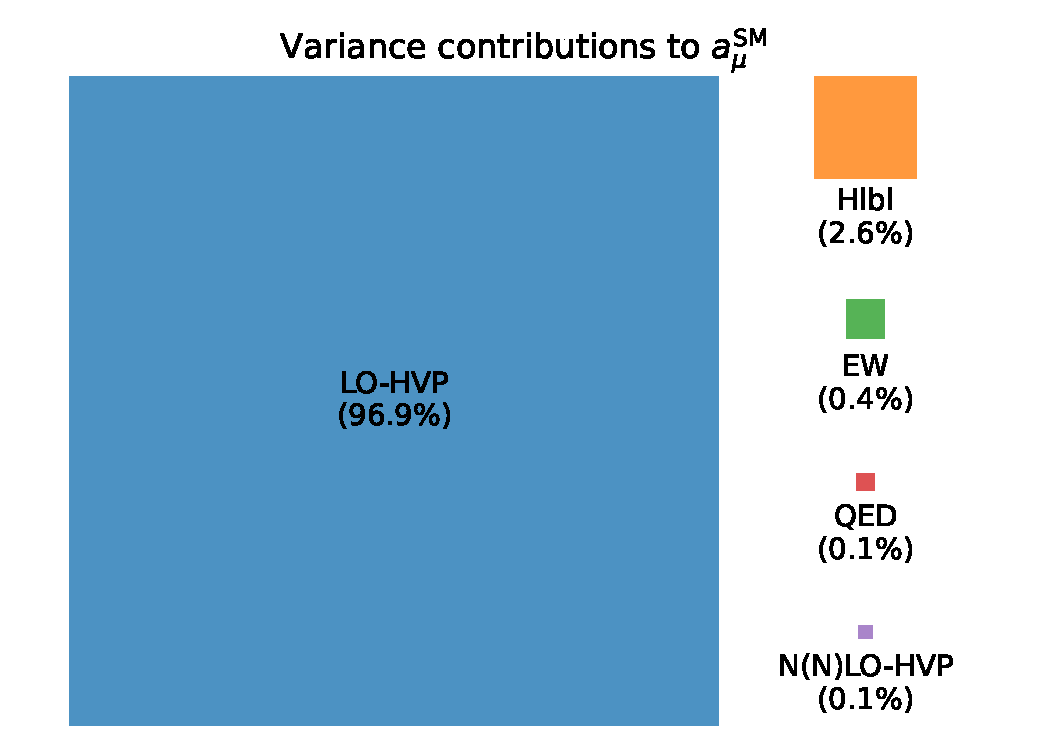
\includegraphics[scale=0.5]{\dir/img/a_mu_sm_variances_squares} % 8
\caption{
Variance contributions to $a_{\mu}^{\text{SM}}$; the official Standard Model prediction to the anomalous magnetic moment of the muon $g-2$.
The areas are proportional to the variances, whereas the side lengths are proportional to the errors.
The contributions stand for: LO-HVP: lattice determination of the leading order HVP contribution (the one we deal with in this thesis), HlBl: mixed (phenomenology and lattice) result for the hadronic light-by-light contribution up to next-to-leading order (NLO), EW: electro-weak contribution, QED: quantum electrodynamics contribution up to tenth order, N(N)LO-HVP: phenomenological result of higher order terms of the HVP.
Data for this plot was taken from ref.~\cite{snowmass:2025}.
}
\label{fig:a_mu:sm:variances}
\end{figure}

\begin{figure}
\centering
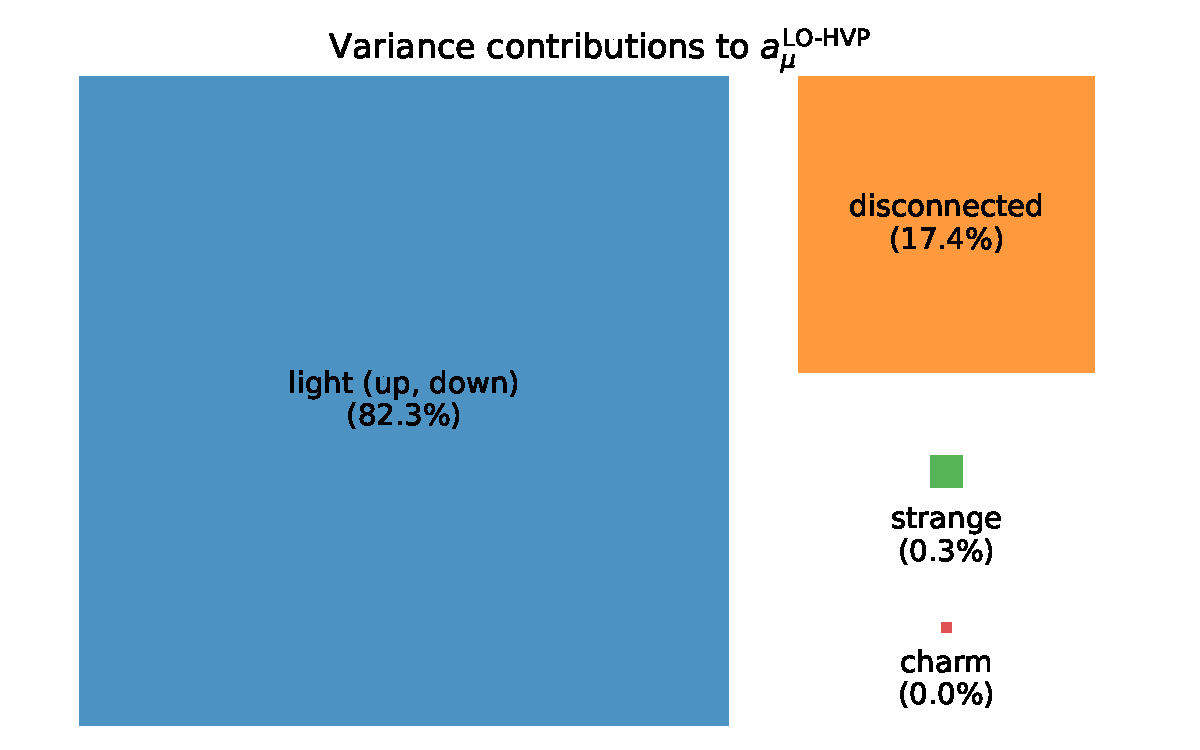
\includegraphics[scale=0.5]{\dir/img/a_mu_lohvp_variances_squares}
\caption{
Variance contributions to $a_{\mu}^{\text{LO-HVP}}$ (blue square in \cref{fig:a_mu:sm:variances}); the official Standard Model prediction to the leading order hadronic vacuum polarization contribution to the anomalous magnetic moment of the muon $g-2$.
The areas are proportional to the variances, whereas the side lengths are proportional to the errors.
The contributions stand for: light: light quark connected contribution (the one we deal with in this thesis), disconnected: sum of all disconnected flavor contributions, strange/charm: contribution of the strange/charm quark flavor.
Data for this plot was taken from ref.~\cite{snowmass:2025}.
}
\label{fig:a_mu:lohvp:variances}
\end{figure}

\tldr{motivation of QCD+QED}
Looking at a different decomposition of $a_{\mu}^{\text{LO-HVP}}$ into window contributions, \cref{eq:a:mu:lohvp:windows}, and IB corrections
\begin{equation}
a_{\mu}^{\text{LO-HVP}} = a_{\mu}^{\text{SD}} + a_{\mu}^{\text{W}} + a_{\mu}^{\text{LD}} + a_{\mu}^{\text{IB}} \;,
\end{equation}
where here the isospin-symmetric component was decomposed into windows and a remainder accounts for the first order strong and QED isospin-breaking corrections due to the mass difference between up and down quarks and QED effects.
For the variance contributions, we find \cref{fig:a_mu:windows:variances}.
Again, the dominant overall contribution comes from the large distance regime (LD) where the signal-to-noise ratio problem is severe, but also from the IB contribution.
Contributions to the value of $a_{\mu}^{\text{LO-HVP}}$ from these effects are expected to the in the 1\% regime, but we see dramatic variance contribution.
Good prescriptions to add QED dynamically to the simulation, rather than perturbatively to a QCD-only simulation afterwards, are thus desperately needed.
First results suggest that errors decrease by a factor of \num{3}, when doing so~\citeOwn{qcd_qed_paola}.

\begin{figure}
\centering
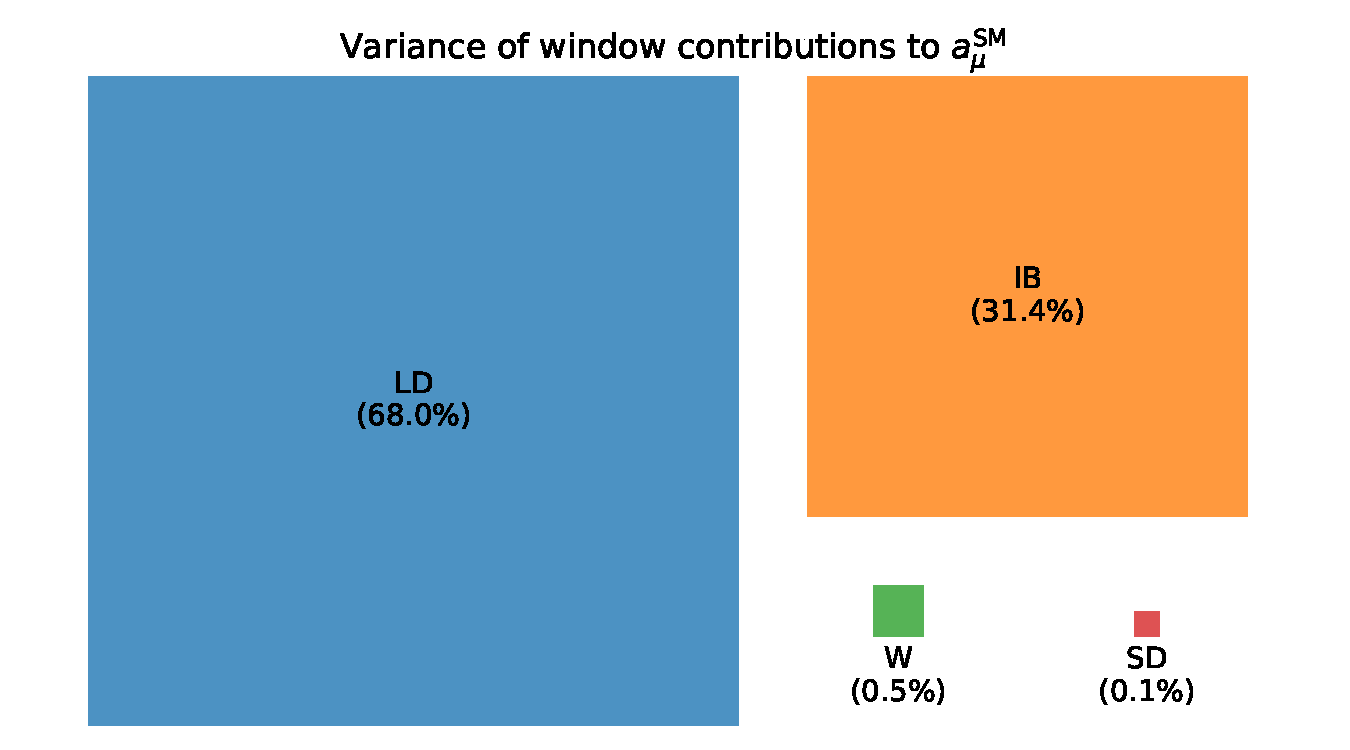
\includegraphics[scale=0.5]{\dir/img/a_mu_windows_variances_squares}
\caption{
Variance contribution if the windows to $a_{\mu}^{\text{LO-HVP}}$ (blue square in \cref{fig:a_mu:sm:variances}).
The areas are proportional to the variances, whereas the side lengths are proportional to the errors.
The contributions stand for: LD: long-distance window, IB: strong and QED isospin-breaking corrections, W: intermediate window, SD: short-distance window.
Data for this plot was taken from ref.~\cite{snowmass:2025}.
}
\label{fig:a_mu:windows:variances}
\end{figure}

\subsection{Efficient usage of HPC resources}

Since modern HPC infrastructure tend towards massively parallel GPU systems or heterogeneous machines, research in computational sciences has the responsibility to utilize these new compute resources efficiently and sensibly.
If that does not happen a stagnation of the field is inevitable.
Efficient usage is only possible if current lattice gauge theory simulation frameworks are utilizing the GPU.
As available pure-CPU compute resources are decreasing yearly, it is expected for them to vanish entirely in the not so far future.
Enabling \openqxd to run on GPUs thus opens important doors for the \RCstar collaboration and lays crucial groundwork for future software developments.
It is evident that HPC hardware continues to change\footnote{An example for a new hardware trend is the intelligence processing unit~\cite{ipu} (IPU) specially designed for machine learning workloads.}.
As soon as the GPU is harvested in terms of efficient usage, the HPC community may continue with practicing heterogeneous computing -- it already does.
Therefore, we explored into this area as well.

In current world politics, energy consumption is more important than ever.
This obligates us as researchers to treat the resources we are allowed to use with extra care, specially in the field of computational lattice field theory -- one of the biggest consumers of HPC.

As important as software developments and efficient utilization of available resources are, the field will not advance without algorithmic developments.
Specially methods to systematically and iteratively improve estimations of observables by reducing their variance are pivotal for numerical high precision determinations of physical quantities.
As traditional estimators either break down or become prohibitively expensive as we approach large, physical lattices, we need efficient variance reduction methods using the available resources more efficiently.

Summarizing the motivation, all aspects of this thesis crucially aim to maximize physics output, while minimizing cost in terms of computational resources and energy.







\section{Thesis objectives and scope}
\label{sec:intro:objectives}

This thesis aims to focus on the following objectives:
\begin{itemize}
   \item Design and efficient implementation to offload of expensive solves of the Dirac equation to the GPU. This includes dealing with \Cstar boundary conditions and QCD+QED Dirac operators as of \cref{eq:Dw:QCD+QED}. This should be done in a modular and versatile fashion for convenient usage for application-level developers and lay foundation for future developments.
   \item Performance assessment and benchmark of all implemented features on target HPC infrastructure including GPUs.
   \item Establishment of a CI/CD automated testing pipeline running on target hardware and production problems.
   \item Algorithmic development of variance reduction methods based on the low-mode deflation technique targeted at observables sensitive to low-mode noise suffering from the signal-to-noise ratio problem.
   \item Theoretical understanding of spectral properties of Dirac operators and their coarse-grid variants.
\end{itemize}
The above objectives all target efficient evaluation of observables from a machine-centric but also from an algorithmic perspective.

The scope of these developments concerns offloading inversions to the GPU and does not extend generally to the generation of gauge configurations, although design decisions were made with that in mind.
A direct proposal for a direct continuation of the software developments in the direction of gauge field generation is stated in \cref{ch:p1:memory}, it is not the only possibility to continue.
Benchmarks are restricted to systems with NVIDIA GPUs, because of availability of compute resources, although data for AMD GPUs has been investigated too, taken on the Finnish machine \emph{LUMI}.
Some of this can be found in ref.~\citeOwn{lattice24:roman} and currently unpublished in ref.~\citeOwn{pasc24}, where also data from the decommissioned \emph{Daint hybrid} machine at CSCS can be found.
This data is from an old version of the code and was therefore left out of this document.

The first part of this document is dedicated to the advancements in software development by interfacing the simulation program \openqxd with \quda.
The foundation of this work was my master's thesis~\citeOwn{lattice21:master_thesis,pasc23} and it is partially based on refs.~\citeOwn{pasc24,lattice24:roman}.

The second part investigates variance reduction using low-mode deflation techniques and is based on refs.~\citeOwn{mglma,lattice23:lma}.
Some of the plots and illustrations presented in this thesis were taken from ref.~\citeOwn{mglma}.
If so, it is indicated specifically in the captions.

A path not further pursued during my PhD was the evaluation of the leading order HVP of the muon $g-2$ using \Cstar boundary conditions and QCD+QED gauge ensembles.
Publications related to this can be found in refs.~\citeOwn{lattice22:roman,lattice22:paola,lattice22:alessandro,lattice22:jens,qcd_qed_paola}.



\section{Summary of contributions}

In this section, I declare my own achievements and contributions to this thesis according to article \num{13} of \cite{eth:doctorate:stipulations}.
I wrote all chapters myself.
I received valuable feedback from colleagues and collaborators, which helped improve the presentation and clarity of this thesis.
All figures, plots and images were produced by me.
Some were taken from the publication~\cite{mglma}.

\begin{description}
\item[\cref{ch:introduction}]: This chapter is introductory, based on established literature and does not contain original research.
\item Part I: GPU Porting of Dirac Solvers
   \begin{description}
   \item[\cref{ch:p1:introduction}]: This chapter is introductory, is based on established literature and does not contain original research.
   \item[\cref{ch:p1:openqxd}]: I compiled this chapter based on access to the source code of \openqxd and its documentation. No original results are presented here.
   \item[\cref{ch:p1:quda}]: I compiled this chapter based on access to the source code of \quda and its documentation. No original results are presented here.
   \item[\cref{ch:p1:interface,ch:p1:develop}]: These chapters describe the software components I developed as part of this project. I was responsible for implementing the core functionality of interfacing \openqxd with \quda. The design of the code was discussed and refined in collaboration with members of the \RCstar collaboration, CSCS engineers and group member related to the PASC project~\cite{online:pasc2025}. The latter also contributed to specific components and architectural decisions. All documentation and the write-up of this chapter were done by me.
   %\item[\cref{ch:p1:develop}]: \worktodo{todo}
   \item[\cref{ch:p1:performance}]: This chapter shows performance data of interface components. I conducted all related runs independently and the analysis of data was done by me. Feedback from members of the \RCstar collaboration was incorporated.
   \item[\cref{ch:p1:cicd}]: The automated testing pipeline was designed and introduced to the development repository~\cite{gitlab:openqxd-devel} by me. CSCS engineers were involved in consultation for best practices.
   \item[\cref{ch:p1:memory}]: The memory management proposal was developed by me and a small proof-of-concept program was written by me too.
   \item[\cref{ch:p1:conclusions}]: This chapter was written by me and reflects my own views and conclusions.
   \end{description}
\item Part II: Variance Reduction for Two-Point Functions
   \begin{description}
   \item[\cref{ch:p2:introduction}]: This chapter is introductory, is based on established literature and does not contain original research.
   \item[\cref{ch:p2:2pt-corr}]: This chapter introduces the relevant formulae required later. Apart from notation, no original results are presented here.
   \item[\cref{ch:p2:lma}]: This chapter introduces the important variance reduction method low-mode averaging and some of its many variants. No original results are presented here.
   \item[\cref{ch:p2:subspace-deflation}]: The novelty in this chapter is the deflation of arbitrary subspaces required later.
   \item[\cref{ch:p2:lc}]: Local coherence is a concept known in literature. This chapter briefly introduces the concept. No original results are presented here.
   \item[\cref{ch:p2:multigrid}]: Multigrid preconditioning is an established concept and widely used in the field. The original research consists of the decomposition of the propagator, its usage as variance reduction method and developments that follow. This was developed by me based on advise and feedback of colleagues and collaborators.
   \item[\cref{ch:p2:numerics}]: I have developed the observable evaluation code, the recursive multigrid and all results were generated by me. The gauge fields used for the numerical analysis of the method, apart from the lattice F7~\cite{online:cls}, were generated by Tim Harris. Feedback from my supervisor Marina Marinković and Tim Harris helped improve the simulation strategy.
   \item[\cref{ch:p2:chirality}]: Theoretical insight from this chapter are my own. Textbook results from numerical range theory were used, but also indicated if so. Ideas about preservation of chirality are partially based on existing literature.
   \item[\cref{ch:p2:conclusions}]: This chapter was written by me and reflects my own views and conclusions.
   \end{description}
\item[\cref{ch:summary}]: This chapter was written by me and reflects my own views and conclusions.
\end{description}

% The main contributions of this thesis are as follows:

% \begin{enumerate}
%    \item \textbf{GPU integration into \openqxd}: Development of a feature to offload inversions to the solver suite of \quda into the core components of \openqxd targeted at observable evaluation. Implementation of \Cstar boundary conditions and the QCD+QED Wilson-Clover Dirac operator in \quda.
%    \item \textbf{Versatile interface API}: Development of useful features such as the dual process grid (\cref{sec:interface:openqxd:dual}) or the asynchronous solver (\cref{sec:interface:solver:async}) allowing heterogeneous computing. The API was designed for easy porting of existing programs in \openqxd that aim to leverage solvers on the GPU.
%    \item \textbf{Performance evaluation}: Performance of all implemented features was carefully measured on state-of-the-art HPC infrastructure and real-world production problems and setups.
%    \item \textbf{CI/CD testing pipeline}: Integration of a CI/CD pipeline into the Git development-repository of \openqxd~\cite{gitlab:openqxd-devel} running on local compute resources as well as on GH200 nodes at CSCS.
%    \item \textbf{Field memory management proposal}: Design and proof-of-concept test of a memory management system to minimize CPU-GPU field transfers useful for a continuation of this work considering gauge field generation.
%    \item \textbf{Development of a novel variance reduction method}: Development, implementation and assessment of a new method called \emph{multigrid low-mode averaging} for $\bigO(a)$-improved Wilson-type fermions, and application of such to the evaluation of the leading order connected light-quark HVP of the muon $g-2$.
%    \item \textbf{Theoretical considerations of chirality}: Investigation and analysis of chirality, spectral properties, numerical ranges and conditions of coarse and fine Dirac operators.
% \end{enumerate}

\section{Structure of the thesis}

This document is split into two parts which are to a large extent independent of each other but pulling on the same rope.
\Cref{part:gpu} deals with the advancements in software development, GPU porting and the interface to \quda.
It deals with \worktodo{contributions \numrange{1}{5}}.
Its heart piece provides a documentation of the design choices, all the functionality that have entered the codebase, and finishes with an assessment of performance.
\Cref{part:variance} deals with the remaining \worktodo{contributions \numrange{6}{7}}, introduces the new variance reduction method which we call \emph{multigrid low-mode averaging} and investigates its application to an observable that is sensitive to it.
Results are compared to traditional estimators.
It finishes with theoretical considerations about chirality on coarse subspaces.
Both parts have separate outlines and introductions.
